\title[EMI, thermal design and integration]{EMI, thermal design and integration}
\section{EMI, thermal and integration}

\begin{frame}[plain]
	\titlepage
\end{frame}

%%%%%%%%%%%%%%%%%%%%%%%%%%%%%%%%%%%%%%%%%%%%%%%%%%%%%%%%%%%%%
%% Overview %%
%%%%%%%%%%%%%%%%%%%%%%%%%%%%%%%%%%%%%%%%%%%%%%%%%%%%%%%%%%%%%
\subsection{EMI fundamentals}

\begin{frame}
	\frametitle{Overview}
	A converter that works on the bench must also pass the EMI test and survive its own heat. Both get harder and easier at the same time when $f_\mathrm{sw}$ rises.
	\begin{itemize}
		\item Conducted and radiated emission, the LISN, limit lines
		\item Spectrum of trapezoidal waveforms; differential and common mode
		\item Mitigation: layout, shielding, $\mathrm{d}v/\mathrm{d}t$, filters and their parasitics
		\item Thermal networks, spreading, transient impedance, electro-thermal feedback
		\item Loss budget, derating and integration trends
	\end{itemize}
	After this lecture you can estimate the spectrum of a switching node, size a filter corner from a required attenuation, and predict the hot-spot temperature of your design.
\end{frame}

%%%%%%%%%%%%%%%%%%%%%%%%%%%%%%%%%%%%%%%%%%%%%%%%%%%%%%%%%%%%%
%% Conducted and radiated %%
%%%%%%%%%%%%%%%%%%%%%%%%%%%%%%%%%%%%%%%%%%%%%%%%%%%%%%%%%%%%%
\begin{frame}
	\frametitle{Conducted and radiated emission}
	\begin{columns}[T]
		\begin{column}{0.5\textwidth}
			\small
			\begin{itemize}
				\item Conducted emission: voltage at the mains or DC terminals, measured with a line impedance stabilisation network (LISN, 50\,$\Omega$/50\,$\mu$H, CISPR 16-1-2) from 150\,kHz to 30\,MHz (CISPR 32, multimedia and ICT equipment).
				\item Radiated emission: field strength from 30\,MHz upwards.
				\item Vehicle components: CISPR 25 with its own bands and limits.
				\item The EMI receiver has quasi-peak and average detectors with 9\,kHz bandwidth in the conducted band. A steady harmonic gives the same reading in both, so the lower average limit decides.
			\end{itemize}
		\end{column}
		\begin{column}{0.47\textwidth}
			\begin{table}
				\centering
				\scriptsize
				\begin{tabular}{|l|c|c|}
					\hline
					$f$ (MHz)  & quasi-peak (dB$\mu$V) & average (dB$\mu$V) \\
					\hline
					0.15--0.5  & 66 to 56              & 56 to 46           \\
					0.5--5     & 56                    & 46                 \\
					5--30      & 60                    & 50                 \\
					\hline
				\end{tabular}
				\caption{Conducted limits at the mains port, class B (residential); the limit falls linearly with $\log f$ between 0.15 and 0.5\,MHz}
			\end{table}
			\small
			Class A (non-residential) allows 79 and 73\,dB$\mu$V quasi-peak, below and above 0.5\,MHz.
		\end{column}
	\end{columns}
	\blfootnote{Sources: CISPR 32, CISPR 16-1-2; H.\,W. Ott, \textit{Electromagnetic Compatibility Engineering}, Wiley, 2009.}
\end{frame}

%%%%%%%%%%%%%%%%%%%%%%%%%%%%%%%%%%%%%%%%%%%%%%%%%%%%%%%%%%%%%
%% LISN %%
%%%%%%%%%%%%%%%%%%%%%%%%%%%%%%%%%%%%%%%%%%%%%%%%%%%%%%%%%%%%%
\begin{frame}
	\frametitle{The LISN}
	\begin{columns}[T]
		\begin{column}{0.5\textwidth}
			\begin{figure}
				\centering
				\begin{circuitikz}[scale=0.8, transform shape]
					\draw (0,0) to[V, l=mains] (0,3) to[L, l=50\,$\mu$H] (3,3) node[circ]{} -- (5.4,3) to[generic, l=EUT] (5.4,0) -- (0,0);
					\draw (3,3) to[C, l_=0.1\,$\mu$F] (3,1.5) to[R, l_={50\,$\Omega$ receiver}] (3,0) node[circ]{};
					\draw (1.5,0) node[ground]{};
				\end{circuitikz}
				\caption{One line of the LISN: above 150\,kHz the equipment sees the 50\,$\Omega$ input of the receiver; the inductor decouples the mains}
			\end{figure}
		\end{column}
		\begin{column}{0.47\textwidth}
			\footnotesize
			\begin{itemize}
				\item The LISN gives the equipment a defined source impedance, independent of the building wiring: measurements become reproducible.
				\item Each line (L and N, or + and $-$) is measured against the reference ground.
				\item A differential-mode (DM) current $i_\mathrm{DM}$, out in one line and back in the other, gives $\pm50\,\Omega\cdot i_\mathrm{DM}$ on the two lines. A common-mode (CM) current $i_\mathrm{CM}$ (sum of both lines, returning through ground) gives $25\,\Omega\cdot i_\mathrm{CM}$ in phase on both.
				\item 56\,dB$\mu$V (the quasi-peak limit from 0.5 to 5\,MHz) correspond to 0.63\,mV, i.e.\ 13\,$\mu$A in 50\,$\Omega$.
			\end{itemize}
		\end{column}
	\end{columns}
	\blfootnote{Source: Ott, 2009, Ch.\ 17; C.\,R. Paul, \textit{Introduction to Electromagnetic Compatibility}, 2nd ed., Wiley, 2006.}
\end{frame}

%%%%%%%%%%%%%%%%%%%%%%%%%%%%%%%%%%%%%%%%%%%%%%%%%%%%%%%%%%%%%
%% Trapezoid spectrum %%
%%%%%%%%%%%%%%%%%%%%%%%%%%%%%%%%%%%%%%%%%%%%%%%%%%%%%%%%%%%%%
\begin{frame}
	\frametitle{Spectrum of a trapezoid}
	\begin{columns}[T]
		\begin{column}{0.47\textwidth}
			\small
			A trapezoidal pulse train with amplitude $A$, pulse width $\tau=DT_\mathrm{s}$ and rise time $t_\mathrm{r}$ has its harmonics below an envelope that is
			\begin{itemize}
				\item flat at $2A\tau/T_\mathrm{s}=2AD$ up to $1/(\pi\tau)$,
				\item $-20$\,dB/decade up to $1/(\pi t_\mathrm{r})$,
				\item $-40$\,dB/decade above.
			\end{itemize}
			The harmonics lie only at multiples of $f_\mathrm{sw}$. A higher $f_\mathrm{sw}$ at the same $D$ shortens $\tau$ and moves the first corner up; the rise time sets the second corner.

			\vspace{0.2cm}
			The limit lies 80 to 90\,dB below the switch-node envelope: input capacitor, filter and the small coupling capacitances must provide this together.
		\end{column}
		\begin{column}{0.5\textwidth}
			\begin{figure}
				\centering
				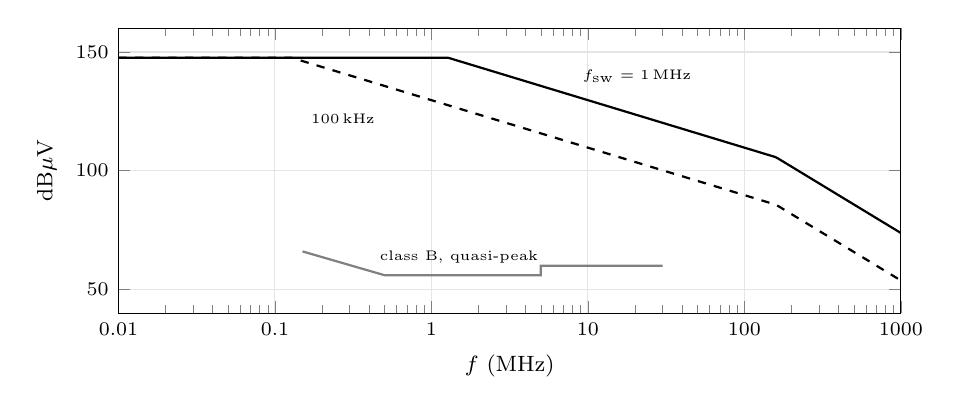
\begin{tikzpicture}
					\begin{semilogxaxis}[
							width=0.95\linewidth, height=5.2cm,
							xmin=0.01, xmax=1000, ymin=40, ymax=160,
							xtick={0.01,0.1,1,10,100,1000}, xticklabels={0.01,0.1,1,10,100,1000},
							xlabel={$f$ (MHz)}, ylabel={dB$\mu$V},
							grid=major, grid style={gray!20},
							tick label style={font=\scriptsize}, label style={font=\footnotesize},
						]
						\addplot[black, thick, domain=-2:3, samples=300] ({10^x}, {147.6 - 20*log10(max(1,10^x/1.273)) - 20*log10(max(1,10^x/159.2))});
						\addplot[black, thick, dashed, domain=-2:3, samples=300] ({10^x}, {147.6 - 20*log10(max(1,10^x/0.1273)) - 20*log10(max(1,10^x/159.2))});
						\addplot[gray, thick] coordinates {(0.15,66) (0.5,56) (5,56) (5,60) (30,60)};
						\node[font=\tiny, anchor=south west] at (axis cs:8,133) {$f_\mathrm{sw}=1$\,MHz};
						\node[font=\tiny, anchor=north east] at (axis cs:0.5,128) {100\,kHz};
						\node[font=\tiny, anchor=south] at (axis cs:1.5,57) {class B, quasi-peak};
					\end{semilogxaxis}
				\end{tikzpicture}
				\caption{Envelope of the harmonics of a 48\,V switch node ($D=0.25$, $t_\mathrm{r}=2$\,ns) at two switching frequencies; grey: class B quasi-peak limit}
			\end{figure}
		\end{column}
	\end{columns}
	\blfootnote{Sources: Paul, 2006, Ch.\ 3; Ott, 2009.}
\end{frame}

%%%%%%%%%%%%%%%%%%%%%%%%%%%%%%%%%%%%%%%%%%%%%%%%%%%%%%%%%%%%%
%% Task: spectrum corners %%
%%%%%%%%%%%%%%%%%%%%%%%%%%%%%%%%%%%%%%%%%%%%%%%%%%%%%%%%%%%%%
% Two pages: task (page 1) and task with solution (page 2).
\begin{frame}<handout:1-2>
	\frametitle{Spectrum corners}
	\begin{block}{Task (2 minutes)}
		A switch node of 48\,V has a pulse width of $\tau=100$\,ns and edges of $t_\mathrm{r}=2$\,ns.
		\begin{enumerate}
			\item Where are the two corners of the envelope?
			\item By how much does the envelope fall from 10\,MHz to 30\,MHz? And if $t_\mathrm{r}$ becomes 10\,ns?
		\end{enumerate}
	\end{block}
	\onslide<2-|handout:2>{
		\begin{enumerate}
			\item $1/(\pi\tau)=3.2$\,MHz and $1/(\pi t_\mathrm{r})=159$\,MHz.
			\item Between the corners $-20$\,dB/decade: $20\log_{10}3=9.5$\,dB. With 10\,ns the second corner moves to 32\,MHz: in the conducted band nothing changes, above 32\,MHz the radiated range gains up to 14\,dB of margin. Slower edges help radiated emission; conducted emission needs the filter.
		\end{enumerate}
	}
\end{frame}

%%%%%%%%%%%%%%%%%%%%%%%%%%%%%%%%%%%%%%%%%%%%%%%%%%%%%%%%%%%%%
%% DM and CM %%
%%%%%%%%%%%%%%%%%%%%%%%%%%%%%%%%%%%%%%%%%%%%%%%%%%%%%%%%%%%%%
\begin{frame}
	\frametitle{Differential and common mode}
	\begin{columns}[T]
		\begin{column}{0.48\textwidth}
			\small
			\textbf{Differential mode (DM)}
			\begin{itemize}
				\item The pulsed input current divides between the input capacitor and the source: ripple current between the lines.
				\item Set by $\mathrm{ESR}$, $\mathrm{ESL}$ and the capacitance of the input capacitors (L3).
			\end{itemize}
			\textbf{Common mode (CM)}
			\begin{itemize}
				\item Every fast node charges its parasitic capacitance $C_\mathrm{p}$ to earth: $i_\mathrm{CM}=C_\mathrm{p}\,\mathrm{d}v/\mathrm{d}t$, returning through the LISN.
				\item Example: switch node to heat sink 20\,pF, 50\,V/ns: 1\,A for the duration of the edge.
			\end{itemize}
		\end{column}
		\begin{column}{0.48\textwidth}
			\small
			\textbf{Parasitic capacitances}
			\begin{itemize}
				\item Switch-node copper and the drain tab to the heat sink or chassis.
				\item Transformer inter-winding capacitance (L7): the main CM path of isolated converters.
				\item Inductor and choke winding capacitance bypass the filter (L7).
			\end{itemize}
			\begin{block}{Key message}
				DM noise follows the current loop, CM noise follows $\mathrm{d}v/\mathrm{d}t$ and stray capacitance.
			\end{block}
		\end{column}
	\end{columns}
	\blfootnote{Sources: Ott, 2009; S. Wang, in Kizilyalli et al.\ (eds.), \textit{Wide Bandgap Power Electronics}, Springer, 2025, ch.\ 20.}
\end{frame}

%%%%%%%%%%%%%%%%%%%%%%%%%%%%%%%%%%%%%%%%%%%%%%%%%%%%%%%%%%%%%
%% MHz moves the problem %%
%%%%%%%%%%%%%%%%%%%%%%%%%%%%%%%%%%%%%%%%%%%%%%%%%%%%%%%%%%%%%
\begin{frame}
	\frametitle{EMI at MHz switching frequency}
	\begin{columns}[T]
		\begin{column}{0.48\textwidth}
			\small
			\textbf{Harder}
			\begin{itemize}
				\item Above 150\,kHz the fundamental lies in the conducted band; the filter must attenuate it directly.
				\item More edges per second, faster edges with GaN: more energy above 30\,MHz.
				\item Parasitics of filter parts limit the attenuation where it is needed.
			\end{itemize}
		\end{column}
		\begin{column}{0.48\textwidth}
			\small
			\textbf{Easier}
			\begin{itemize}
				\item A filter corner scales with the frequency to be attenuated: smaller $L$ and $C$.
				\item 30\,W LED driver at 5 to 10\,MHz meets FCC class B; the whole converter is smaller than the EMI filter of a conventional design.
				\item 250\,W PFC supply at 1 to 4\,MHz, 95.3\,\% at full load: EMI filter 8\,\% of the box volume.
			\end{itemize}
		\end{column}
	\end{columns}
	\begin{block}{Key message}
		At MHz the EMI filter is not a burden but one of the gains, if its parasitics are designed in.
	\end{block}
	\blfootnote{Source: Perreault, APEC 2024 plenary, citing S. Lim et al., IEEE TPEL 2016, and J. Santiago-Gonzalez et al., IEEE JESTIE 2023.}
\end{frame}

%%%%%%%%%%%%%%%%%%%%%%%%%%%%%%%%%%%%%%%%%%%%%%%%%%%%%%%%%%%%%
%% Mitigation at the source %%
%%%%%%%%%%%%%%%%%%%%%%%%%%%%%%%%%%%%%%%%%%%%%%%%%%%%%%%%%%%%%
\subsection{EMI mitigation}

\begin{frame}
	\frametitle{Mitigation at the source}
	\begin{columns}[T]
		\begin{column}{0.48\textwidth}
			\small
			\begin{itemize}
				\item Small commutation loop with the return in the adjacent layer (L3): less ringing, less radiated field.
				\item Small switch-node area; a shield layer connected to the quiet DC rail between switch node and heat sink returns the CM current locally.
				\item Transformers: shield windings and symmetric winding arrangements (L7).
			\end{itemize}
		\end{column}
		\begin{column}{0.48\textwidth}
			\small
			\begin{itemize}
				\item Soft switching: ZVS edges are set by $C_\mathrm{oss}$ and current, no ringing at turn-on (L8).
				\item $\mathrm{d}v/\mathrm{d}t$ control by the gate resistor costs switching loss (L4).
				\item Balanced topologies: two switch nodes with opposite $\mathrm{d}v/\mathrm{d}t$ cancel their CM currents.
				\item Spread spectrum: frequency modulation spreads each harmonic over more 9\,kHz receiver bins and lowers the reading; it does not lower the energy.
			\end{itemize}
		\end{column}
	\end{columns}
	\blfootnote{Sources: Ott, 2009; Wang, 2025.}
\end{frame}

%%%%%%%%%%%%%%%%%%%%%%%%%%%%%%%%%%%%%%%%%%%%%%%%%%%%%%%%%%%%%
%% DM filter %%
%%%%%%%%%%%%%%%%%%%%%%%%%%%%%%%%%%%%%%%%%%%%%%%%%%%%%%%%%%%%%
\begin{frame}
	\frametitle{Filter design}
	\begin{columns}[T]
		\begin{column}{0.5\textwidth}
			\footnotesize
			One $LC$ stage attenuates with 40\,dB/decade above its corner. For an attenuation $A$ (dB) needed at $f_x$:
			\begin{equation*}
				f_\mathrm{c}=f_x\cdot10^{-A/40},\qquad L=\frac{Z}{2\pi f_\mathrm{c}},\quad C=\frac{1}{2\pi f_\mathrm{c}Z}
			\end{equation*}
			with a chosen characteristic impedance $Z=\sqrt{L/C}$; two stages for more than about 60\,dB.
		\end{column}
		\begin{column}{0.47\textwidth}
			\footnotesize
			\begin{itemize}
				\item Damping: a regulated converter draws constant power and thus has a negative incremental input resistance $-V^2/P$. The filter output impedance must stay well below $V^2/P$ at all frequencies (Middlebrook), or filter and converter oscillate. An $R$--$C$ damper across the filter capacitor limits the resonance peak.
				\item CM filter: a CM choke (the DM fluxes of its two windings cancel, so it does not saturate) and Y capacitors to earth, whose value the touch current limits.
				\item Above the self-resonance a choke is a capacitor and a capacitor an inductor: split windings, parallel capacitors, short connections.
			\end{itemize}
		\end{column}
	\end{columns}
	\blfootnote{Sources: Erickson and Maksimovi\'c, 2020, Ch.\ 17; Ott, 2009.}
\end{frame}

%%%%%%%%%%%%%%%%%%%%%%%%%%%%%%%%%%%%%%%%%%%%%%%%%%%%%%%%%%%%%
%% Task: filter corner %%
%%%%%%%%%%%%%%%%%%%%%%%%%%%%%%%%%%%%%%%%%%%%%%%%%%%%%%%%%%%%%
% Two pages: task (page 1) and task with solution (page 2).
\begin{frame}<handout:1-2>
	\frametitle{Filter corner from the attenuation}
	\begin{block}{Task (3 minutes)}
		A DM filter must provide 60\,dB at the first harmonic inside the band, with $Z=2\,\Omega$.
		\begin{enumerate}
			\item Corner, $L$ and $C$ for a converter at 1\,MHz?
			\item The same for a converter whose first relevant harmonic lies at 150\,kHz. Ratio of the $LC$ products?
		\end{enumerate}
	\end{block}
	\onslide<2-|handout:2>{
		\begin{enumerate}
			\item $f_\mathrm{c}=1\,\mathrm{MHz}\cdot10^{-1.5}=31.6$\,kHz; $L=10.1\,\mu$H, $C=2.5\,\mu$F.
			\item $f_\mathrm{c}=4.7$\,kHz; $L=67\,\mu$H, $C=17\,\mu$F. The $LC$ product is 44 times larger. Both need damping, and both must keep their attenuation up to 30\,MHz despite the parasitics.
		\end{enumerate}
	}
\end{frame}

%%%%%%%%%%%%%%%%%%%%%%%%%%%%%%%%%%%%%%%%%%%%%%%%%%%%%%%%%%%%%
%% Poll: CM path %%
%%%%%%%%%%%%%%%%%%%%%%%%%%%%%%%%%%%%%%%%%%%%%%%%%%%%%%%%%%%%%
% Two pages: question (page 1) and guidance (page 2).
\begin{frame}<handout:1-2>
	\frametitle{Your common-mode path}
	\begin{columns}[T]
		\begin{column}{0.48\textwidth}
			\small
			Poll: which path dominates the common-mode noise of your project design?
			\begin{enumerate}[A]
				\item switch node to heat sink or chassis
				\item transformer inter-winding capacitance
				\item gate driver isolation barrier
				\item cables and the load
			\end{enumerate}
		\end{column}
		\begin{column}{0.48\textwidth}
			\onslide<2-|handout:2>{
				\begin{block}{Guidance}
					Estimate each path with $C_\mathrm{p}\,\mathrm{d}v/\mathrm{d}t$. Non-isolated converters with a heat sink (B1, B3): usually A. Isolated converters (B2): usually B; shield windings help. Gate drivers (C) matter at high $\mathrm{d}v/\mathrm{d}t$ with a few pF of barrier capacitance (L4). WPT (B4): the coil and the receiver form a large antenna, D.
				\end{block}
			}
		\end{column}
	\end{columns}
\end{frame}

%%%%%%%%%%%%%%%%%%%%%%%%%%%%%%%%%%%%%%%%%%%%%%%%%%%%%%%%%%%%%
%% Thermal network %%
%%%%%%%%%%%%%%%%%%%%%%%%%%%%%%%%%%%%%%%%%%%%%%%%%%%%%%%%%%%%%
\subsection{Thermal design}

\begin{frame}
	\frametitle{Thermal network}
	\begin{columns}[T]
		\begin{column}{0.48\textwidth}
			\footnotesize
			Steady state: thermal resistances in series and parallel, losses as current sources. $P$: loss of the device, $P_\mathrm{shared}$: total loss into the common heat sink; $R_\mathrm{jc}$ junction to case, $R_\mathrm{cs}$ case to sink, $R_\mathrm{sa}$ sink to ambient:
			\begin{equation*}
				T_\mathrm{j}=T_\mathrm{a}+P\left(R_\mathrm{jc}+R_\mathrm{cs}+\ldots\right)+P_\mathrm{shared}R_\mathrm{sa}
			\end{equation*}
			\begin{itemize}
				\item Chip-scale GaN: top-side cooling through the die, or bottom-side through solder, thermal vias and the board.
				\item Loss density decides: the same loss in a smaller converter leaves through a smaller surface, so the thermal resistance must be lower.
			\end{itemize}
		\end{column}
		\begin{column}{0.48\textwidth}
			\footnotesize
			\textbf{Thermal vias}: drill $d=0.3$\,mm, plating $t=25\,\mu$m, board $l=1.6$\,mm, copper $k=390$\,W/(m\,K); barrel $A=\pi(d-t)t=0.0216\,\mathrm{mm^2}$:
			\begin{equation*}
				R_\mathrm{via}=\frac{l}{kA}\approx190\,\mathrm{K/W}
			\end{equation*}
			20 vias in parallel: 9.5\,K/W.
			\vspace{0.2cm}

			\textbf{Spreading}: a 70\,$\mu$m copper layer has a sheet thermal resistance $1/(kt)=37$\,K/W per square; heat spreads only a few millimetres around a hot spot.
		\end{column}
	\end{columns}
	\blfootnote{Sources: Kassakian et al., 2023 (thermal modelling and heat sinking); IEEE EPS Heterogeneous Integration Roadmap 2023, ch.\ 20.}
\end{frame}

%%%%%%%%%%%%%%%%%%%%%%%%%%%%%%%%%%%%%%%%%%%%%%%%%%%%%%%%%%%%%
%% Task: hot spot %%
%%%%%%%%%%%%%%%%%%%%%%%%%%%%%%%%%%%%%%%%%%%%%%%%%%%%%%%%%%%%%
% Two pages: task (page 1) and task with solution (page 2).
\begin{frame}<handout:1-2>
	\frametitle{A 2\,W hot spot}
	\begin{block}{Task (3 minutes)}
		A transistor dissipates 2\,W: junction to board 2\,K/W, 20 thermal vias (9.5\,K/W), interface material to the heat sink 2\,K/W. The heat sink (5\,K/W to ambient) carries the total converter loss of 6\,W; ambient 40\,$^\circ$C.
		\begin{enumerate}
			\item Junction temperature?
			\item Which single change helps most?
		\end{enumerate}
	\end{block}
	\onslide<2-|handout:2>{
		\begin{enumerate}
			\item Heat sink: $40+6\cdot5=70\,^\circ$C. Path: $2\,\mathrm{W}\cdot(2+9.5+2)\,\mathrm{K/W}=27$\,K. $T_\mathrm{j}=97\,^\circ$C.
			\item The vias carry 19\,K of it: 40 vias halve it, copper-filled vias cut it to about a third; top-side cooling bypasses the board. The shared heat sink sets the base: 30\,K.
		\end{enumerate}
	}
\end{frame}

%%%%%%%%%%%%%%%%%%%%%%%%%%%%%%%%%%%%%%%%%%%%%%%%%%%%%%%%%%%%%
%% Transient thermal impedance %%
%%%%%%%%%%%%%%%%%%%%%%%%%%%%%%%%%%%%%%%%%%%%%%%%%%%%%%%%%%%%%
\begin{frame}
	\frametitle{Transient thermal impedance}
	\begin{columns}[T]
		\begin{column}{0.48\textwidth}
			\small
			Foster model fitted to the $Z_\mathrm{th}$ curve of the data sheet ($R_i$, $\tau_i$: fitted pairs):
			\begin{equation*}
				Z_\mathrm{th}(t)=\sum_iR_i\left(1-\mathrm{e}^{-t/\tau_i}\right)
			\end{equation*}
			\begin{itemize}
				\item The die has time constants of microseconds to milliseconds: the ripple at MHz does not appear in the junction temperature, its average does.
				\item Load steps, start-up and short circuits: use $Z_\mathrm{th}(t)$, not $R_\mathrm{th}$.
			\end{itemize}
		\end{column}
		\begin{column}{0.48\textwidth}
			\small
			\begin{itemize}
				\item The Foster network describes the terminal behaviour only; for combining with a heat sink use a Cauer network (physical layers).
				\item Magnetics: large time constants (minutes); hot spot inside the winding or at the gap.
				\item Simulation: thermal networks in SPICE (current sources for losses, capacitances for heat capacity) or FEM for spreading.
			\end{itemize}
		\end{column}
	\end{columns}
	\blfootnote{Source: Kassakian et al., 2023.}
\end{frame}

%%%%%%%%%%%%%%%%%%%%%%%%%%%%%%%%%%%%%%%%%%%%%%%%%%%%%%%%%%%%%
%% Electro-thermal feedback %%
%%%%%%%%%%%%%%%%%%%%%%%%%%%%%%%%%%%%%%%%%%%%%%%%%%%%%%%%%%%%%
\begin{frame}
	\frametitle{Electro-thermal feedback}
	\begin{columns}[T]
		\begin{column}{0.5\textwidth}
			\small
			The loss rises with temperature, $P=P_0\left[1+\alpha(T-T_\mathrm{a})\right]$, and flows through $R_\mathrm{th}$ to the ambient at $T_\mathrm{a}$:
			\begin{equation*}
				\Delta T=\frac{R_\mathrm{th}P_0}{1-\alpha R_\mathrm{th}P_0}
			\end{equation*}
			Stable only for $\alpha R_\mathrm{th}P_0<1$; near 1 the temperature runs away.
			\begin{itemize}
				\item $R_\mathrm{DS(on)}$ of Si and GaN roughly doubles from 25 to 150\,$^\circ$C: $\alpha$ of the order of 0.01/K.
				\item Ferrites have a loss minimum near the design temperature; above it the core loss rises.
			\end{itemize}
		\end{column}
		\begin{column}{0.47\textwidth}
			\small
			Example: $P_0=2$\,W, $R_\mathrm{th}=20$\,K/W, $\alpha=0.008$/K: without feedback 40\,K, with feedback
			\begin{equation*}
				\Delta T=\frac{40\,\mathrm{K}}{1-0.32}=59\,\mathrm{K}
			\end{equation*}
			\begin{block}{Key message}
				Calculate losses at the operating temperature, iterate until temperature and loss agree.
			\end{block}
		\end{column}
	\end{columns}
\end{frame}

%%%%%%%%%%%%%%%%%%%%%%%%%%%%%%%%%%%%%%%%%%%%%%%%%%%%%%%%%%%%%
%% Measuring temperature %%
%%%%%%%%%%%%%%%%%%%%%%%%%%%%%%%%%%%%%%%%%%%%%%%%%%%%%%%%%%%%%
\begin{frame}
	\frametitle{Measuring temperature}
	\begin{columns}[T]
		\begin{column}{0.48\textwidth}
			\small
			\begin{itemize}
				\item Thermocouples: cheap and small, but metallic: on a switch node they pick up noise and can short a node; glue them with insulating adhesive.
				\item Infrared camera: field view; emissivity of copper, solder mask and GaN dies differs, so cover with matte black paint or tape of known emissivity.
			\end{itemize}
		\end{column}
		\begin{column}{0.48\textwidth}
			\small
			\begin{itemize}
				\item Fibre-optic sensors: immune to $\mathrm{d}v/\mathrm{d}t$ and fields, for windings and high-voltage nodes.
				\item Temperature-sensitive electrical parameters such as $R_\mathrm{DS(on)}$ or a body-diode drop measure the junction itself (L5).
				\item Calorimetric loss measurement closes the energy balance (L5).
			\end{itemize}
		\end{column}
	\end{columns}
\end{frame}

%%%%%%%%%%%%%%%%%%%%%%%%%%%%%%%%%%%%%%%%%%%%%%%%%%%%%%%%%%%%%%
%% Loss budget %%
%%%%%%%%%%%%%%%%%%%%%%%%%%%%%%%%%%%%%%%%%%%%%%%%%%%%%%%%%%%%%
\subsection{Loss budget and integration}

\begin{frame}
	\frametitle{The loss budget}
	\begin{table}
		\centering
		\scriptsize
		\begin{tabular}{|l|>{\raggedright\arraybackslash}p{5.2cm}|>{\raggedright\arraybackslash}p{4.6cm}|c|}
			\hline
			\textbf{Element}     & \textbf{Model}                                                        & \textbf{Uncertainty}                              & \textbf{Lecture} \\
			\hline
			conduction           & $I_\mathrm{rms}^2R_\mathrm{DS(on)}(T)$, dynamic $R_\mathrm{DS(on)}$    & temperature, current collapse of GaN              & L2               \\
			switching            & overlap, $Q_\mathrm{oss}V$ or partial ZVS, reverse conduction         & dead time, nonlinear $C_\mathrm{oss}$, hysteresis & L2, L8           \\
			gate drive           & $Q_\mathrm{G}V_\mathrm{GS}f_\mathrm{sw}$ plus driver bias             & driver data at frequency                          & L4               \\
			core                 & iGSE with the real waveform, at temperature                           & material data, temperature                        & L6               \\
			winding              & Dowell, proximity, termination                                        & field near the gap, layout                        & L7               \\
			capacitors           & $I_\mathrm{rms}^2\,\mathrm{ESR}$                                      & ESR at frequency and temperature                  & L3, L12          \\
			PCB and connectors   & $I^2R$ of copper at temperature                                       & current crowding                                  & L3               \\
			control, sensing     & bias power, shunts                                                    & small, but fixed                                  & L13              \\
			\hline
		\end{tabular}
		\caption{Template of the loss budget for milestone M4}
	\end{table}
	\small
	Sensitivity: vary each uncertain parameter by its tolerance and show which one moves the efficiency most; that is the measurement to plan first.
\end{frame}

%%%%%%%%%%%%%%%%%%%%%%%%%%%%%%%%%%%%%%%%%%%%%%%%%%%%%%%%%%%%%
%% Derating %%
%%%%%%%%%%%%%%%%%%%%%%%%%%%%%%%%%%%%%%%%%%%%%%%%%%%%%%%%%%%%%
\begin{frame}
	\frametitle{Derating and component selection}
	\begin{columns}[T]
		\begin{column}{0.48\textwidth}
			\small
			\begin{itemize}
				\item Voltage: margin above the worst-case peak including ringing and nonlinear $C_\mathrm{oss}$ (Tutorial 10: 98\,V peak in a class E at 24\,V).
				\item Temperature: junction and hot-spot limits with margin for ambient and ageing; electrolytic capacitors halve their life per 10\,K.
				\item Capacitance at DC bias, temperature and age (L12).
			\end{itemize}
		\end{column}
		\begin{column}{0.48\textwidth}
			\small
			\begin{itemize}
				\item Magnetics: saturation at the highest temperature and current, including transients.
				\item Company and application rules (automotive, industrial) fix the margins; state yours explicitly in the design package.
			\end{itemize}
			\begin{block}{Key message}
				A design is only as good as its worst corner: every rating is checked at the corner where it is stressed most.
			\end{block}
		\end{column}
	\end{columns}
\end{frame}

%%%%%%%%%%%%%%%%%%%%%%%%%%%%%%%%%%%%%%%%%%%%%%%%%%%%%%%%%%%%%
%% Integration %%
%%%%%%%%%%%%%%%%%%%%%%%%%%%%%%%%%%%%%%%%%%%%%%%%%%%%%%%%%%%%%
\begin{frame}
	\frametitle{Integration trends}
	\begin{columns}[T]
		\begin{column}{0.48\textwidth}
			\small
			\begin{itemize}
				\item Switching cell in the package: driver, transistors and decoupling in one module; the commutation loop shrinks to the package (L3, L4).
				\item Power system-in-package and embedded dies in the PCB: shorter loops, double-sided cooling.
				\item Integrated voltage regulators on or near the processor: FIVR and vertical power delivery (L11).
			\end{itemize}
		\end{column}
		\begin{column}{0.48\textwidth}
			\small
			\begin{itemize}
				\item Power supply on chip (PwrSoC): magnetics on silicon or in the package; the frequency rises to tens of MHz to make them small.
				\item Thermal management and magnetic materials remain the bottlenecks named by the roadmap.
			\end{itemize}
			\begin{block}{Key message}
				Integration turns the parasitic problems of L3 into design parameters, and the heat into the main limit.
			\end{block}
		\end{column}
	\end{columns}
	\blfootnote{Sources: IEEE EPS Heterogeneous Integration Roadmap 2023, ch.\ 10 and 20; C. \'O Math\'una et al., IEEE TPEL, vol.\ 27, no.\ 11, 2012.}
\end{frame}

%%%%%%%%%%%%%%%%%%%%%%%%%%%%%%%%%%%%%%%%%%%%%%%%%%%%%%%%%%%%%
%% Briefs %%
%%%%%%%%%%%%%%%%%%%%%%%%%%%%%%%%%%%%%%%%%%%%%%%%%%%%%%%%%%%%%
\begin{frame}
	\frametitle{EMI and heat in the briefs}
	\begin{table}
		\centering
		\footnotesize
		\begin{tabular}{|l|>{\raggedright\arraybackslash}p{3.0cm}|>{\raggedright\arraybackslash}p{9.6cm}|}
			\hline
			   & \textbf{Brief}           & \textbf{Question from this lecture}                                                                              \\
			\hline
			B1 & ZVS GaN buck, 1--3\,MHz  & fundamental in the band; variable $f_\mathrm{sw}$ spreads the spectrum; GaN hot spot through the board           \\
			B2 & LLC DCX, 1\,MHz          & transformer inter-winding capacitance as CM path; SR and transformer heat                                         \\
			B3 & DAB, 0.5--1\,MHz         & two switch nodes, CM through the transformer; thermal balance of both bridges                                     \\
			B4 & 6.78\,MHz class E        & ISM band, harmonics and radiated emission of the coil; heat in the matching inductor                              \\
			B5 & 13.56\,MHz VHF           & harmonics up to the radiated range; air-core stray fields; small parts, high loss density                         \\
			B6 & hybrid SC, 48\,V         & input current pulses (DM); capacitor heating by rms current                                                        \\
			\hline
		\end{tabular}
		\caption{Milestone M4 (03.02.): EMI estimate and thermal check of the final design}
	\end{table}
\end{frame}

%%%%%%%%%%%%%%%%%%%%%%%%%%%%%%%%%%%%%%%%%%%%%%%%%%%%%%%%%%%%%
%% Key messages %%
%%%%%%%%%%%%%%%%%%%%%%%%%%%%%%%%%%%%%%%%%%%%%%%%%%%%%%%%%%%%%
\begin{frame}
	\frametitle{Key messages}
	\begin{enumerate}
		\item Conducted emission is measured with the 50\,$\Omega$/50\,$\mu$H LISN from 150\,kHz to 30\,MHz; above that the radiated range begins.
		\item The trapezoid envelope is flat to $1/(\pi\tau)$, falls by 20\,dB/decade to $1/(\pi t_\mathrm{r})$ and by 40\,dB/decade above.
		\item DM follows the current loop, CM follows $C_\mathrm{p}\,\mathrm{d}v/\mathrm{d}t$; shields and balance act at the source.
		\item A filter corner scales with the frequency to be attenuated: MHz converters need smaller filters, with designed parasitics and damping.
		\item Thermal design: series resistances from junction to ambient, vias of about 190\,K/W each, electro-thermal feedback.
		\item The loss budget at operating temperature, with its sensitivities, decides what to measure first.
	\end{enumerate}
\end{frame}

%%%%%%%%%%%%%%%%%%%%%%%%%%%%%%%%%%%%%%%%%%%%%%%%%%%%%%%%%%%%%
%% Exit ticket %%
%%%%%%%%%%%%%%%%%%%%%%%%%%%%%%%%%%%%%%%%%%%%%%%%%%%%%%%%%%%%%
% Two pages: questions (page 1) and answers (page 2).
\begin{frame}<handout:1-2>
	\frametitle{Exit questions}
	\begin{varblock}[\textwidth]{Three questions, one minute each}
		\begin{enumerate}
			\item Edges of 1\,ns: where does the $-40$\,dB/decade region begin?
			\item Why does a common-mode choke hardly attenuate differential-mode current?
			\item $P_0=3$\,W, $R_\mathrm{th}=15$\,K/W, $\alpha=0.01$/K: temperature rise with feedback?
		\end{enumerate}
	\end{varblock}
	\onslide<2-|handout:2>{
		\begin{enumerate}
			\item $1/(\pi\cdot1\,\mathrm{ns})=318$\,MHz.
			\item The DM currents flow in opposite directions through the two windings; their fluxes cancel. Only the leakage inductance acts on DM.
			\item $\alpha R_\mathrm{th}P_0=0.45$: $\Delta T=45\,\mathrm{K}/0.55=82$\,K instead of 45\,K.
		\end{enumerate}
	}
\end{frame}

%%%%%%%%%%%%%%%%%%%%%%%%%%%%%%%%%%%%%%%%%%%%%%%%%%%%%%%%%%%%%
%% References %%
%%%%%%%%%%%%%%%%%%%%%%%%%%%%%%%%%%%%%%%%%%%%%%%%%%%%%%%%%%%%%
\begin{frame}
	\frametitle{References}
	\scriptsize
	\begin{itemize}
		\item H.\,W. Ott, \textit{Electromagnetic Compatibility Engineering}, Wiley, 2009.
		\item C.\,R. Paul, \textit{Introduction to Electromagnetic Compatibility}, 2nd ed., Wiley, 2006.
		\item CISPR 32, \textit{Electromagnetic compatibility of multimedia equipment -- Emission requirements}; CISPR 16-1-2 (coupling devices for conducted disturbance measurements); CISPR 25 (vehicles).
		\item R.\,W. Erickson, D. Maksimovi\'c, \textit{Fundamentals of Power Electronics}, 3rd ed., Springer, 2020, Ch.\ 17.
		\item J.\,G. Kassakian, D.\,J. Perreault, G.\,C. Verghese, M.\,F. Schlecht, \textit{Principles of Power Electronics}, 2nd ed., Cambridge University Press, 2023.
		\item S. Wang, ``Characteristics, challenges, and solutions to electromagnetic interference in wide bandgap semiconductor power electronics systems,'' in Kizilyalli et al.\ (eds.), \textit{Wide Bandgap Power Electronics}, Springer, 2025, ch.\ 20.
		\item IEEE Electronics Packaging Society, \textit{Heterogeneous Integration Roadmap}, 2023 edition, ch.\ 10 (Integrated Power Electronics) and ch.\ 20 (Thermal).
		\item C. \'O Math\'una, N. Wang, S. Kulkarni, S. Roy, ``Review of integrated magnetics for power supply on chip (PwrSoC),'' IEEE Trans.\ Power Electron., vol.\ 27, no.\ 11, pp.\ 4799--4816, 2012.
		\item D.\,J. Perreault, ``Opportunities, progress and challenges in high-frequency power conversion,'' plenary talk, IEEE APEC 2024.
	\end{itemize}
\end{frame}
